En un modelo adimensional de equilibrio térmico se cumple \(u_{xx}+u_{yy}=0\) en el cuadrado \(0<x<3\), \(0<y<3\). Se usa una malla de paso uno en ambas direcciones. Los valores de contorno son sintéticos; las cuatro incógnitas interiores aparecen en la tabla:
\[
\begin{array}{c|rrrr}
y\backslash x&0&1&2&3\\\hline
3&4&7&12&19\\
2&8&C&D&23\\
1&10&A&B&25\\
0&10&13&18&25
\end{array}
\]
Aproxime cada derivada segunda mediante la diferencia centrada correspondiente; por ejemplo,
\[
u_{xx}(i,j)\approx U_{i+1,j}-2U_{i,j}+U_{i-1,j}.
\]
Construya y resuelva el sistema para \(A,B,C,D\). Como referencia, examine el polinomio
\[
H(x,y)=x^2-y^2+2x+y+10.
\]
Compruebe su relación con la ecuación y los datos de la tabla, compare sus valores interiores con la solución del sistema y explique el alcance de ese acuerdo.

\Needspace{11.91cm}
\begin{center}
\begin{minipage}{\linewidth}
\centering
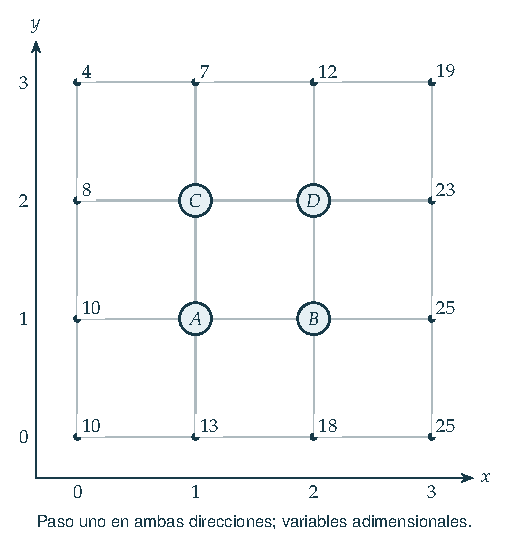
\includegraphics[width=9.66cm]{assets/M2-E0356-setup.pdf}\par
\smallskip{\small Posición de los datos de contorno y de las cuatro incógnitas interiores.\par}
\end{minipage}
\end{center}
